\documentclass[a4paper,10pt]{article}

\usepackage{tikz}
\usepackage{fullpage}
\usepackage{amsmath,amsthm,amsfonts,amssymb,amscd}
\usepackage{mathtools}
\usepackage{colortbl}
\usepackage{xcolor}
\usepackage{graphicx}
\usepackage{titlesec}
\usepackage{xepersian}
\usepackage{multirow}
\usepackage{caption}
\usepackage{fancyhdr}
\usepackage{mdframed}


% ---------------------------
%      Color Palette
% ---------------------------
\definecolor{BgDark}{HTML}{141420}
\definecolor{BgCard}{HTML}{1E1E2E}
\definecolor{AccentBlue}{HTML}{7AA2F7}
\definecolor{AccentPurple}{HTML}{BB9AF7}
\definecolor{AccentCyan}{HTML}{7DCFFF}
\definecolor{AccentGold}{HTML}{E0AF68}
\definecolor{TextPrimary}{HTML}{CDD6F4}
\definecolor{TextMuted}{HTML}{6C7086}
\definecolor{RuleLine}{HTML}{313244}

\pagecolor{BgDark}
\color{TextPrimary}


% ---------------------------
%  RTL-safe Info Box
% ---------------------------
\newmdenv[
backgroundcolor=BgCard,
fontcolor=TextPrimary,
linecolor=AccentBlue,
linewidth=1.2pt,
rightline=true,   % RTL: accent border on the RIGHT
leftline=false,
topline=false,
bottomline=false,
innerrightmargin=12pt,
innerleftmargin=12pt,
innertopmargin=10pt,
innerbottommargin=10pt,
skipabove=10pt,
skipbelow=10pt,
]{infobox}
% ---------------------------
%        Font Setup
% ---------------------------
\settextfont{Vazir.ttf}[
    BoldFont = Vazir-Bold.ttf,
    Path = fonts/
]
\setlatintextfont{Vazir.ttf}[
    BoldFont = Vazir-Bold.ttf,
    Path = fonts/
]

% ---------------------------
%     Custom Adjustments
% ---------------------------
\renewcommand{\baselinestretch}{1.2}
\renewcommand{\thesection}{\arabic{section}}

% User-defined commands for homework info (adjust as needed)
\newcommand{\HomeworkNumber}{4}
\newcommand{\HomeworkDeadline}{1405/02/12}
\newcommand{\id}{\texttt{\detokenize{@Mohammad_Bagher_Mahdizadeh}}}



\begin{document}

% ---------------------------------
%           Title Page
% ---------------------------------
\begin{titlepage}
	
	% Background decorations — right-side rectangle + gold horizontal line
	\begin{tikzpicture}[remember picture, overlay]
		% Right-side vertical rectangle (accent block)
		\fill[BgCard]
		([xshift=-2.2cm]current page.north east) rectangle
		(current page.south east);
		\draw[AccentGold!60, line width=0.8pt]
		([xshift=-2.2cm]current page.north east) --
		([xshift=-2.2cm]current page.south east);
	\end{tikzpicture}
	
	\vspace*{2.2cm}
	
	\begin{center}
		% Logo
		
\includegraphics[scale=1.05]{assets/fum-logo.png}\\[1.0cm]
		
		\textcolor{RuleLine}{\rule{8cm}{0.6pt}}\\[0.6cm]
		
		{\Huge \bfseries \textcolor{TextPrimary}{مبانی و کاربردهای هوش مصنوعی}}\\[0.4cm]
		
		\textcolor{RuleLine}{\rule{8cm}{0.6pt}}\\[0.4cm]
		
		{\large \textcolor{AccentCyan}{دانشگاه فردوسی مشهد}}\\[0.1cm]
		{\normalsize \textcolor{TextMuted}{گروه مهندسی کامپیوتر}}\\[0.2cm]
		{\normalsize \textcolor{AccentGold}{دکتر زارعی}}\\[1.6cm]
		{\normalsize \textcolor{TextMuted}{بهار 1405}}\\[0.2cm]
		
		% Homework number — simple, normal size
		{\normalsize \textcolor{TextMuted}{تمرین شماره}}
		{\large \bfseries \textcolor{AccentBlue}{\HomeworkNumber}}\\[1.4cm]
		
		% Deadline badge — gold border
		\setlength{\fboxrule}{0.8pt}%
		\fcolorbox{AccentGold!60}{BgCard}{%
			\begin{minipage}{7cm}
				\centering\vspace{5pt}
				\textcolor{AccentGold}{\bfseries مهلت تحویل: \HomeworkDeadline}
				\vspace{5pt}
			\end{minipage}
		}\\[0.8cm]
		
		% TA box — gold border
		\fcolorbox{AccentGold!60}{BgCard}{%
			\begin{minipage}{8cm}
				\centering\vspace{5pt}
				\textcolor{TextMuted}{مسئول تمرین:} \quad \textcolor{AccentCyan}{\id}
				\vspace{5pt}
			\end{minipage}
		}
	\end{center}
	
\end{titlepage}
% ---------------------------------
%          Instructions Page
% ---------------------------------
\clearpage

\vspace*{4pt}
\begin{center}
	\colorbox{BgCard}{%
		\begin{minipage}{\dimexpr\linewidth-2\fboxsep\relax}
			\centering
			\vspace{6pt}
			{\bfseries\large \textcolor{AccentGold}{دستورالعمل‌ها}}
			\vspace{6pt}
		\end{minipage}%
	}
\end{center}
\vspace{6pt}

\begin{infobox}
	دانشجویان محترم لطفا به موارد زیر توجه فرمایید:
	\begin{itemize}
		\itemsep0.4em
		\item
		تحویل تمرین‌ها فقط از طریق سامانه آموزش مجازی دانشگاه امکان‌پذیر است.
		\item
		تمرین‌ها باید دست‌نویس، خوانا و با استفاده از خودکار آبی یا مشکی و یا به صورت دیجیتالی با استفاده از قلم نوری نوشته شوند.
		\item
		از تمرین‌های حل‌شده دیگران استفاده نکنید. پیامدهای این کار با دانشجو می‌باشد.
		\item
		نوشتن جواب آخر به تنهایی نمره‌ای نداشته و تمام مراحل حل، مشمول نمره می‌باشد.
		\item
		به دلیل موعد از پیش تعیین‌شده تمرین‌ها و برنامه درسی، امکان تمدید تمرین وجود ندارد. همچنین ارسال تمرین پس از موعد تعیین‌شده نمره‌ای نخواهد داشت.
		\item
		نحوه نام‌گذاری فایل پاسخ باید مطابق جدول~\ref{tab:file_format} و به شکل \lr{\texttt{pdf}} باشد.
	\end{itemize}
	
	\vspace{10pt}
	
	% RTL-safe table: use center environment, manual column colors
	\begin{center}
		\arrayrulecolor{RuleLine}
		\begin{tabular}{|>{\columncolor{BgCard}\centering\arraybackslash}p{3cm}|>{\columncolor{BgDark}\centering\arraybackslash}p{7cm}|}
			\hline
			\textcolor{AccentCyan}{\bfseries\lr{Format}} &
			\texttt{\lr{StudentID-Full\_Name-\#HwNo.pdf}} \\
			\hline
			\textcolor{AccentGold}{\bfseries\lr{Example}} &
			\textcolor{TextMuted}{\texttt{\lr{9876543210-Alan\_Turing-\#01.pdf}}} \\
			\hline
		\end{tabular}
		\captionof{table}{\textcolor{TextMuted}{شیوه نام‌گذاری فایل‌ها}}
		\label{tab:file_format}
	\end{center}
	
\end{infobox}


\vspace{8pt}
\textcolor{AccentCyan}{\rule{\linewidth}{0.8pt}}
% ---------------------------------
%          questions
% ---------------------------------
%%%%%%%%%%%%%%%%%%%%%%%%%%%%%%%%%%%%%%%%%%%%%%%%%%%%%%%%%%%%%%%%%%%%%%%%%%%%%%%%%%%%%%%%%%%%%%
\section{\textcolor{AccentGold}{سوال اول}}

مفاهیم گراف حالات، درخت جست‌وجو و درخت بازی را تعریف کنید. 

\bigskip
\bigskip
\textcolor{AccentCyan}{\rule{\linewidth}{0.4pt}}
%%%%%%%%%%%%%%%%%%%%%%%%%%%%%%%%%%%%%%%%%%%%%%%%%%%%%%%%%%%%%%%%%%%%%%%%%%%%%%%%%%%%%%%%%%%%%%
\section{\textcolor{AccentGold}{سوال دوم}}

در این سوال به بررسی مفاهیم پایه در این فصل بوسیله بررسی بازی tic-tac-toe می‌پردازید. تابع ارزیابی  به شرح زیر است:

\begin{infobox}
	%Here I want the explanations about notations in evaluation function like X_n, O_n and the evaluation function itself
	% the problem is using both english letters and persian sentences to gether while keeping them neat and aligned 
	\[
	Eval(s) = 3X_2 + X_1 - ( 3O_2 + O_1 )
	\]
	
	\begin{itemize}
		\item 
		\(X_n\): 
		تعداد قطرها، سطرها و ستون‌های بدون O که تعداد X ها در آنها دقیقا \(n\) می‌باشد.
		
		\item 
		\(O_n\): 
		تعداد قطرها، سطرها و ستون‌های بدون X که تعداد O ها در آنها دقیقا \(n\) می‌باشد.
	\end{itemize}
	
\end{infobox}

\begin{enumerate}
	\renewcommand{\labelenumi}{\textcolor{AccentCyan}{\arabic{enumi})}}
	\item 
	درخت بازی را از ابتدای بازی و با شروع مهره  \lr{X}، برای یک دور از بازی‌ ( دو نوبت ) رسم کنید. برای هر گره، فرزاندانی که با یکدیگر قرینه هستند را یک گره فرض کنید.  
	\item 
	مقدار تابع ارزیابی را برای گره‌های در عمق دو مشخص کنید.
	\item 
	باتوجه به مقادیر بدست آمده در مرحله قبل، مقدار backed up را برای گره‌ها با عمق یک و صقر مشخص کنید. با استفاده از این مقادیر، بهترین انتخاب را علامت بزنید. 
	\item 
	با فرض اینکه گره‌ها ترتیب کاملا مطلوبی دارند، نشان دهید که با استفاده از alpha-beta pruning کدام گره‌ها قبل از بررسی حذف می‌شوند. 
\end{enumerate}

\bigskip
\bigskip
\textcolor{AccentCyan}{\rule{\linewidth}{0.4pt}}
%%%%%%%%%%%%%%%%%%%%%%%%%%%%%%%%%%%%%%%%%%%%%%%%%%%%%%%%%%%%%%%%%%%%%%%%%%%%%%%%%%%%%%%%%%%%%%
\section{\textcolor{AccentGold}{سوال سوم}}

فرض کنید در یک بازی دو نفره، نوبتی، قطعی، با اطلاعات کامل و مجموع-ثابت، بازیکن MAX از راهبرد minimax استفاده می‌کند. نشان دهید اگر بازیکن MIN در برخی گره‌ها حرکتی غیر از حرکت بهینه‌ی خود انتخاب کند، مقدار نهایی MAX کمتر از مقدار تضمین‌شده توسط minimax نخواهد شد(توضیح مفهومی کافی است). 

آیا اگر MAX بداند که رقیب در چه موقعیت‌هایی غیر بهینه بازی می‌کند، ممکن است با انتخاب راهبردی غیر از minimax به نتیجه‌ی بهتری برسد؟ با یک مثال توضیح دهید.

\bigskip
\bigskip
\textcolor{AccentCyan}{\rule{\linewidth}{0.4pt}}
%%%%%%%%%%%%%%%%%%%%%%%%%%%%%%%%%%%%%%%%%%%%%%%%%%%%%%%%%%%%%%%%%%%%%%%%%%%%%%%%%%%%%%%%%%%%%%
\section{\textcolor{AccentGold}{سوال چهارم}}

توضیح دهید که ترتیب بازدید گره‌ها جه تاثیری بر عملکرد \lr{alpha-beta pruning} دارد. آیا در صورتی که این ترتیب کاملا مطلوب باشد  استفاده از \lr{ alpha-beta pruning} منطقی است؟ جست‌و‌جو چطور؟ چرا؟ 

\bigskip
\bigskip
\textcolor{AccentCyan}{\rule{\linewidth}{0.4pt}}
%%%%%%%%%%%%%%%%%%%%%%%%%%%%%%%%%%%%%%%%%%%%%%%%%%%%%%%%%%%%%%%%%%%%%%%%%%%%%%%%%%%%%%%%%%%%%%
\section{\textcolor{AccentGold}{سوال پنچم}}

به سوالات زیر با ذکر دلیل پاسخ دهید:

\begin{enumerate}
	\renewcommand{\labelenumi}{\textcolor{AccentCyan}{\arabic{enumi}}}
	\item 
	در نبود شرط \lr{Zero Sum} اما برقراری شرط \lr{constant sum} درستی الگوریتم MIN-MAX کلاسیک را تحقیق کنید. 
	\item 
	به طورکلی اگر در یک بازی با دو بازیکن هیچ یک از شروط بالا برقرار نباشند، آیا می‌توان از \lr{alpha-beta pruning} استفاده کرد؟
	\item 
	به طورکلی آیا می‌توان در یک بازی با بیش از دو بازیکن و برقراری یکی از شروط بالا از \lr{alpha-beta pruning} به روش سنتی بهره برد؟
	\item 
	آیا در یک بازی با بیش از دو بازیکن و در نبود دو شرط بالا می‌توان از \lr{alpha-beta pruning} استفاده کرد؟
\end{enumerate}

\bigskip
\bigskip
\textcolor{AccentCyan}{\rule{\linewidth}{0.4pt}}
%%%%%%%%%%%%%%%%%%%%%%%%%%%%%%%%%%%%%%%%%%%%%%%%%%%%%%%%%%%%%%%%%%%%%%%%%%%%%%%%%%%%%%%%%%%%%%
\section{\textcolor{AccentGold}{سوال ششم}}

محدودیت زمانی و حافظه از دلایل اصلی استفاده از توابع \lr{heurisitic} و متوقف کردن جست‌وجو قبل از بررسی تمامی حالات می‌باشد. به دو سوال زیر در این رابطه پاسخ دهید:
\begin{enumerate}
	\renewcommand{\labelenumi}{\textcolor{AccentCyan}{\arabic{enumi}}}
	\item 
	در به کارگیری روش دوم، دو مسئله \lr{non-quiescent positions} و \lr{hoirzon effect} بوجود می‌آیند. این مسائل را تعریف کنید. 
	\item 
	در بسیاری از درخت های بازی‌، پیچیدگی بازی در عمق‌های مختلف یکسان نیست‌( برای مثال \lr{branching factor} مختلف). در این حالت استفاده از یک مقدار ثابت برای عمق برش، \lr{Cut Off value}، می‌تواند به استفاده نادرست از زمان جست‌وجو منجر شود. با بررسی الگوریتم‌های گفته شده در فصول قبل، الگوریتمی را فقط نام ببرید که با بهره‌گیری از آن می‌توان به روشی پویا‌تر برای برش جست‌وجو رسید. 
\end{enumerate}


\bigskip
\bigskip
\textcolor{AccentCyan}{\rule{\linewidth}{0.4pt}}
%%%%%%%%%%%%%%%%%%%%%%%%%%%%%%%%%%%%%%%%%%%%%%%%%%%%%%%%%%%%%%%%%%%%%%%%%%%%%%%%%%%%%%%%%%%%%%
\section{\textcolor{AccentGold}{سوال هفتم (نمره اضافه)}}
پس از مطالعه توضیحاتی که در ادامه آماده است، به دلخواه به یکی از سوالات زیر پاسخ دهید.

\begin{infobox}
	\( Expectiminimax\): 
در بسیاری از بازی‌ها، علاوه بر تصمیم‌های بازیکنان، شانس و عوامل غیرقطعی نیز در نتیجه‌ی بازی دخیل هستند. در مدل‌سازی چنین بازی‌هایی، درخت بازی تنها از گره‌های تصمیم‌گیری بازیکنان تشکیل نمی‌شود؛ بلکه در کنار گره‌های مربوط به بازیکنان، گره‌های شانس نیز ظاهر می‌شوند. در بازی‌های دو نفره، گره‌های تصمیم‌گیری معمولاً با عنوان‌های MAX و MIN نمایش داده می‌شوند، اما در حالت کلی‌تر، هر گره‌ی تصمیم‌گیری می‌تواند نماینده‌ی نوبت یکی از بازیکنان باشد.

گره‌ی شانس زمانی به درخت اضافه می‌شود که ادامه‌ی بازی، نه فقط به تصمیم بازیکن، بلکه به یک رویداد تصادفی نیز وابسته باشد؛ برای نمونه، پرتاب تاس، کشیدن یک کارت، یا وقوع یک نتیجه‌ی احتمالی در محیط. هر یال خروجی از گره‌ی شانس، یکی از پیامدهای ممکن آن رویداد را نشان می‌دهد و با احتمالی متناظر با همان پیامد وزن‌دهی می‌شود. بنابراین مقدار یک گره‌ی شانس، برخلاف گره‌های MAX و MIN، با انتخاب بیشینه یا کمینه تعیین نمی‌شود؛ بلکه برابر امید ریاضی مقدار گره‌های فرزند آن است.

برای مثال، در بازی منچ، نتیجه‌ی حرکت بازیکن تا حدی به عدد تاس وابسته است. در هر نوبت، ابتدا نتیجه‌ی تاس مشخص می‌شود و سپس بازیکن، با توجه به عدد به‌دست‌آمده و وضعیت مهره‌های خود، یکی از حرکت‌های قانونی را انتخاب می‌کند. از این رو، درخت بازی منچ را می‌توان به گونه‌ای مدل‌سازی کرد که در آن گره‌های شانس، نتایج ممکن پرتاب تاس را نشان می‌دهند و پس از هر نتیجه‌ی ممکن، گره‌ی تصمیم‌گیری بازیکن قرار می‌گیرد. به این ترتیب، درخت چنین بازی‌ای علاوه بر گره‌های تصمیم‌گیری بازیکنان، شامل گره‌های شانس با یال‌های وزن‌دار بر اساس احتمال وقوع هر نتیجه نیز خواهد بود.
\end{infobox}

\begin{figure}[h]
	\centering
	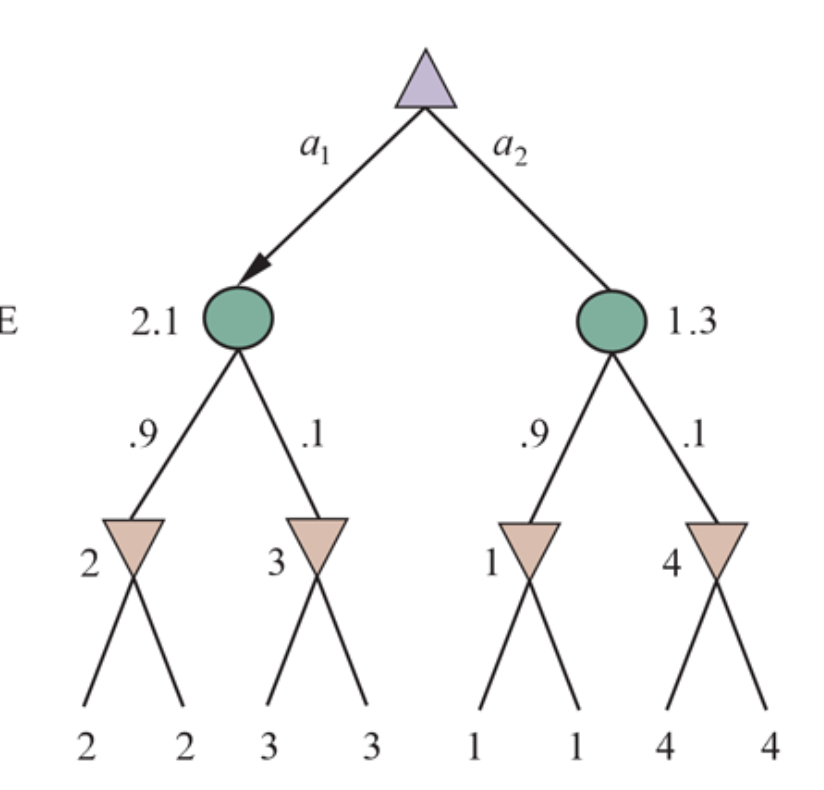
\includegraphics[width=0.5\linewidth]{assets/sample_tree}
	\caption{درخت نمونه}
\end{figure}

\begin{infobox}
	در شکل 1، گره ریشه نشان‌دهنده‌ی نوبت تصمیم‌گیری بازیکن MAX است. این بازیکن می‌تواند یکی از دو عمل \(a_1\) یا \(a_2\) را انتخاب کند. با این حال، پس از انتخاب هر عمل، نتیجه‌ی نهایی به صورت قطعی مشخص نمی‌شود؛ بلکه یک رویداد تصادفی رخ می‌دهد. این رویدادهای تصادفی با گره‌های شانس نمایش داده شده‌اند.
	
	در گره‌های شانس، برخلاف گره‌های MAX و MIN، مقدار گره با گرفتن بیشینه یا کمینه‌ی مقدار فرزندان تعیین نمی‌شود، بلکه برابر امید ریاضی مقدار فرزندان است. به بیان دیگر، مقدار هر فرزند در احتمال رسیدن به آن ضرب می‌شود و سپس این مقادیر با یکدیگر جمع می‌شوند.
	
	برای عمل \(a_1\)، با احتمال \(0.9\) مقدار نهایی \(2\) و با احتمال \(0.1\) مقدار نهایی \(3\) حاصل می‌شود. بنابراین مقدار مورد انتظار این عمل برابر است با:
	\[
	0.9 \times 2 + 0.1 \times 3 = 2.1
	\]
	
	برای عمل \(a_2\)، با احتمال \(0.9\) مقدار نهایی \(1\) و با احتمال \(0.1\) مقدار نهایی \(4\) حاصل می‌شود. بنابراین مقدار مورد انتظار این عمل برابر است با:
	\[
	0.9 \times 1 + 0.1 \times 4 = 1.3
	\]
	
	از آنجا که گره ریشه متعلق به بازیکن MAX است، بازیکن عملی را انتخاب می‌کند که بیشترین ارزش مورد انتظار را داشته باشد. در نتیجه، در این مثال عمل \(a_1\) انتخاب می‌شود، زیرا مقدار مورد انتظار آن، یعنی \(2.1\)، از مقدار مورد انتظار عمل \(a_2\)، یعنی \(1.3\)، بیشتر است.
\end{infobox}

\begin{enumerate}
	\renewcommand{\labelenumi}{\textcolor{AccentCyan}{\arabic{enumi}}}
	\item 
	برای درخت موجود در شکل ۲، مقدار امید ریاضی را برای تمامی گره‌های شانس بدست آورید.پس مشخص کردن مقادیر گره‌های تصمیم، انتخاب MAX را علامت بزنید.
	\item 
	در این سؤال، نسخه‌ای تصادفی و رقابتی از بازی دوز\LTRfootnote{Tic-tac-toe} را بررسی می‌کنیم. در این نسخه، دو صفحه‌ی مستقل از بازی دوز وجود دارد و دو بازیکن، یعنی \(X\) و \(O\)، به نوبت حرکت می‌کنند. در ابتدای هر نوبت، یک سکه پرتاب می‌شود تا مشخص شود بازیکن باید حرکت خود را روی کدام یک از دو صفحه انجام دهد. بازیکنی که زودتر بتواند در یکی از دو صفحه، سه علامت خود را در یک سطر، ستون یا قطر کامل کند، برنده‌ی بازی خواهد بود. در صورت پر شدن تمامی صفحات و برنده نشدن هیچ یک از بازیکنان در یک صفحه، بازیکن شروع کننده بازنده است. 
	
	این بازی را به صورت یک درخت بازی مدل کنید. در توضیح خود مشخص کنید که:
	\begin{itemize}
		\item هر وضعیت بازی شامل چه اطلاعاتی است؛
		\item گره‌های تصمیم‌گیری بازیکنان چه معنایی دارند؛
		\item گره‌های شانس ناشی از پرتاب سکه در کجای درخت قرار می‌گیرند؛
	\end{itemize}
	
\end{enumerate}

\begin{figure}[h]
	\centering
	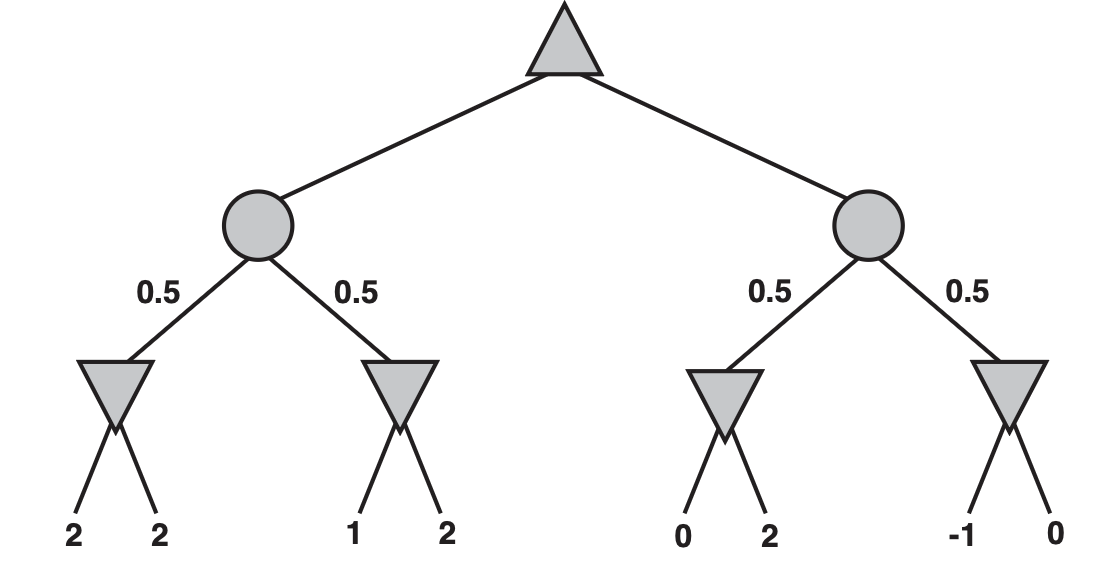
\includegraphics[width=0.5\linewidth]{assets/tree1}
	\caption{درخت سوال هفت-بخش اول}
\end{figure}

\bigskip
\bigskip
\textcolor{AccentCyan}{\rule{\linewidth}{0.4pt}}
%%%%%%%%%%%%%%%%%%%%%%%%%%%%%%%%%%%%%%%%%%%%%%%%%%%%%%%%%%%%%%%%%%%%%%%%%%%%%%%%%%%%%%%%%%%%%%

% Add more sections as needed...

\end{document}
